\documentclass[a4paper,notitlepage]{article}

\usepackage{fullpage}
\usepackage{graphicx}
\usepackage{float}
\usepackage{appendix}
\usepackage{listings}
\usepackage{xcolor}

\definecolor{mGreen}{rgb}{0,0.6,0}
\definecolor{mGray}{rgb}{0.5,0.5,0.5}
\definecolor{mPurple}{rgb}{0.58,0,0.82}
\definecolor{backgroundColour}{rgb}{0.95,0.95,0.92}

\lstdefinestyle{CStyle}{
    backgroundcolor=\color{backgroundColour},
    commentstyle=\color{mGreen},
    keywordstyle=\color{magenta},
    numberstyle=\tiny\color{mGray},
    stringstyle=\color{mPurple},
    basicstyle=\footnotesize,
    breakatwhitespace=false,
    breaklines=true,
    captionpos=b,
    keepspaces=true,
    numbers=left,
    numbersep=5pt,
    showspaces=false,
    showstringspaces=false,
    showtabs=false,
    tabsize=2,
    language=C
}

\renewcommand{\contentsname}{Contenidos}

\begin{document}
\tableofcontents
\section{Resolución}
El árbol de búsqueda binario implementado se basa en la estructura btree{\_}t, la
cual puede representar un nodo de un árbol o un árbol completo según cómo se
lo interprete (root en la función main es el nodo raíz del árbol, pero también
representa al árbol completo). Esta estructura contiene dos punteros a otros
objetos de su mismo tipo que representan la rama izquierda y derecha del nodo,
y también un entero que representa el valor almacenado.

Se implementaron una serie de funciones para interactuar con punteros a btree{\_}t
de modo que un usuario de la estructura no necesite acceder a los miembros de
forma directa. También se implementaron algunas funciones con declaraciones un
poco más específicas para resoluciones de problemas particulares, no se espera
que un usuario utilice estas funciones. Con esa distinción, la lista de
funciones publicas es la siguiente:

\begin{itemize}
    \item btree{\_}new{\_}node
    \item btree{\_}free
    \item btree{\_}search
    \item btree{\_}insert
    \item btree{\_}delete
    \item btree{\_}print
\end{itemize}

Las clases "privadas" que no deberían ser utilizadas por usuarios directamente
son las siguientes:

\begin{itemize}
    \item btree{\_}pop{\_}leaf
    \item btree{\_}replace{\_}node
    \item btree{\_}delete{\_}inner
    \item btree{\_}print{\_}inner
\end{itemize}

En un proyecto más real, btree{\_}t y sus funciones vivirían en un archivo .c
y sólo se expondrían las funciones públicas mediante un .h, por simplicidad
aquí se decidió dejar todo en un mismo archivo fuente.

La documentación para cada función está junto al código en formato doxygen.

\pagebreak

\section{Preguntas}
\subsection{Crear un árbol binario de la siguiente forma.}
\begin{figure}[H]
    \centering
    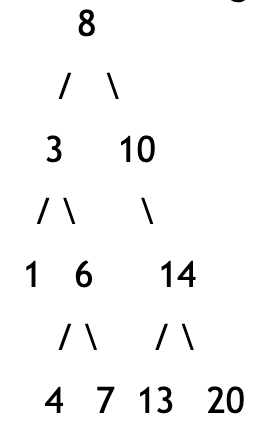
\includegraphics[scale=0.65]{imgs/base-tree.png}
\end{figure}

Para representar el árbol, se eligió un formato distinto en el que los nodos
se imprimen en una forma similar al comando tree. Se puede ver comparando las
representaciones que el subnodo superior en esta representación corresponde
al lado izquierdo del nodo y el inferior al derecho.

\begin{figure}[H]
    \centering
    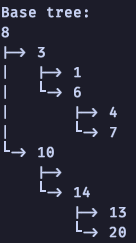
\includegraphics[scale=0.65]{imgs/base-tree-run.png}
\end{figure}

\pagebreak

\subsection{Implementar el método “insertar nodo” e insertar los nodos 24 y 5.}
Tras insertar los nuevos nodos, el 5 se úbica al lado derecho del nodo 4 y el
24 al lado derecho del nodo 20.

\begin{figure}[H]
    \centering
    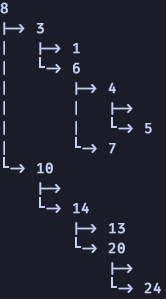
\includegraphics[scale=0.65]{imgs/insert-nodes.png}
\end{figure}

\subsection{Implementar el método “eliminar nodo” y eliminar los nodos 6 y 10.}
Tras eliminar el nodo 6, el nodo 5, que era la hoja más grande de su rama
izquierda, toma su lugar. Al eliminar el nodo 10 y siendo que no tiene rama
izquierda, el nodo 13 toma su lugar por ser la hoja más pequeña de su rama
derecha.

\begin{figure}[H]
    \centering
    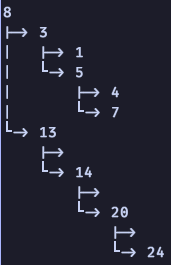
\includegraphics[scale=0.65]{imgs/delete-nodes.png}
\end{figure}

\subsection{Implementar el método “buscar nodo”.}

El método se implementó y a modo de prueba se lo utilizó para imprimir el árbol
a partir del nodo 5

\begin{figure}[H]
    \centering
    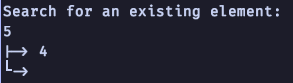
\includegraphics[scale=0.65]{imgs/search.png}
\end{figure}

\subsection{¿Cuál es el valor almacenado en la raíz del árbol?}
La raíz contiene el valor 8 desde la creación del árbol hasta el final del
ejercicio. Sin embargo, en mi código agregué una prueba removiendo la raíz
por ser un caso particular de mi código.

\subsection{¿Cuántos nodos tiene el árbol?}
El árbol tiene 10 nodos al iniciar el ejercicio, sube a 12 al
insertar 5 y 24 y vuelve a 10 tras eliminar 6 y 10.

\subsection{¿Cuál es el valor almacenado en el nodo más a la izquierda del árbol?}
Durante toda la duración del ejercicio, el nodo que está más a la izquierda es
el 1, que también es (lógicamente) el valor más pequeño utilizado en el
ejercicio.

\subsection{¿Cuál es el valor almacenado en el nodo más a la derecha del árbol?}
Durante toda la duración del ejercicio, el nodo que está más a la derecha es
el 24.

\subsection{¿Cuál es la profundidad del árbol?}
El árbol comienza con una profundidad de 4, se incrementa a 5 al insertar los
nodos 24 y 5. La profundidad de 5 se mantiene tras eliminar los nodos 6 y 10.

\begin{appendix}
    \section{Código utilizado}
    \lstinputlisting[style=CStyle]{../src/main.c}
\end{appendix}
\end{document}
